\section{Tests}

TODO: Write about all the snow simulator configurations when doing these tests
Also write about what solvers were used by PETSc and which solver is used
by the default gpu snow simulator

TODO: When running the solver on the cpu the following command line arguments
are given: "\emph{-vec\_type standard -mat\_type aij}" and on the gpu:
"\emph{-vec\_type viennacl -mat\_type aijviennacl}".

\subsection{Convergence Tests}

TODO: Write about the convergence

\subsection{Performance Tests}

\subsubsection{Time Distribution}

This test measures how the execution time of the wind simulation is distributed
between these key functions in the implementation:
\begin{description}
	\item[advect:] Performs the advection step of the wind simulation.
	\item[setupSolution:] Computes the right-hand side of the linear system.
	\item[setInitialGuess:] Sets the initial guess for the solver.
	\item[solve:] Solves the Poisson equation using a PETSc solver.
	\item[project:] Performs the projection step of the wind simulation.
	\item[windToGPU:] Moves the wind velocity field to texture memory for the
	snow particle simulation.
\end{description}

The solver chosen for this test is GMRES, this was specified with the command
line argument "\emph{-ksp\_type gmres}".
This test is performed for four different configurations of the wind simulation:
\begin{description}
	\item[Configuration 1] $ \{ 32, 16, 32 \} $, results are shown in figure
		\ref{fig:td_conf1}
	\item[Configuration 2] $ \{ 64, 32, 64 \} $, results are shown in figure
		\ref{fig:td_conf2} 
	\item[Configuration 3] $ \{ 128, 64, 128 \} $, results are shown in figure
		\ref{fig:td_conf3}
	\item[Configuration 4] $ \{ 256, 128, 256 \} $, results are shown in figure
		\ref{fig:td_conf4}
\end{description}

The results of the time distribution tests is the average execution time of each
key function after 100 frames of simulation.

\begin{figure}[ht]
	\center
	
	\begin{subfigure}{0.45\textwidth}
		\center
		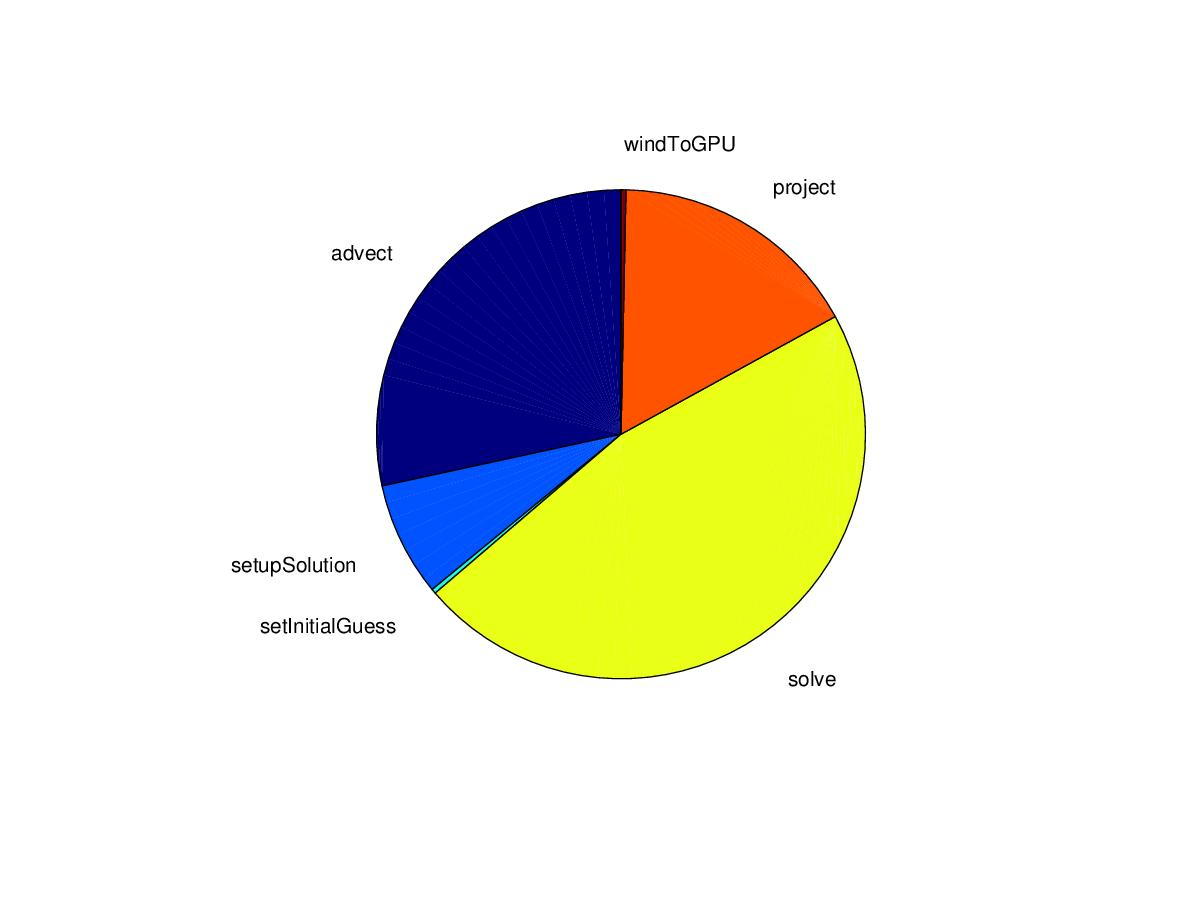
\includegraphics[width=1.0\textwidth]{results/data/td_conf1_petsc_gpu}
		\caption{PETSc on the GPU with OpenCL.}
		\label{fig:td_conf1_petsc_gpu}
	\end{subfigure}
	\begin{subfigure}{0.45\textwidth}
		\center
		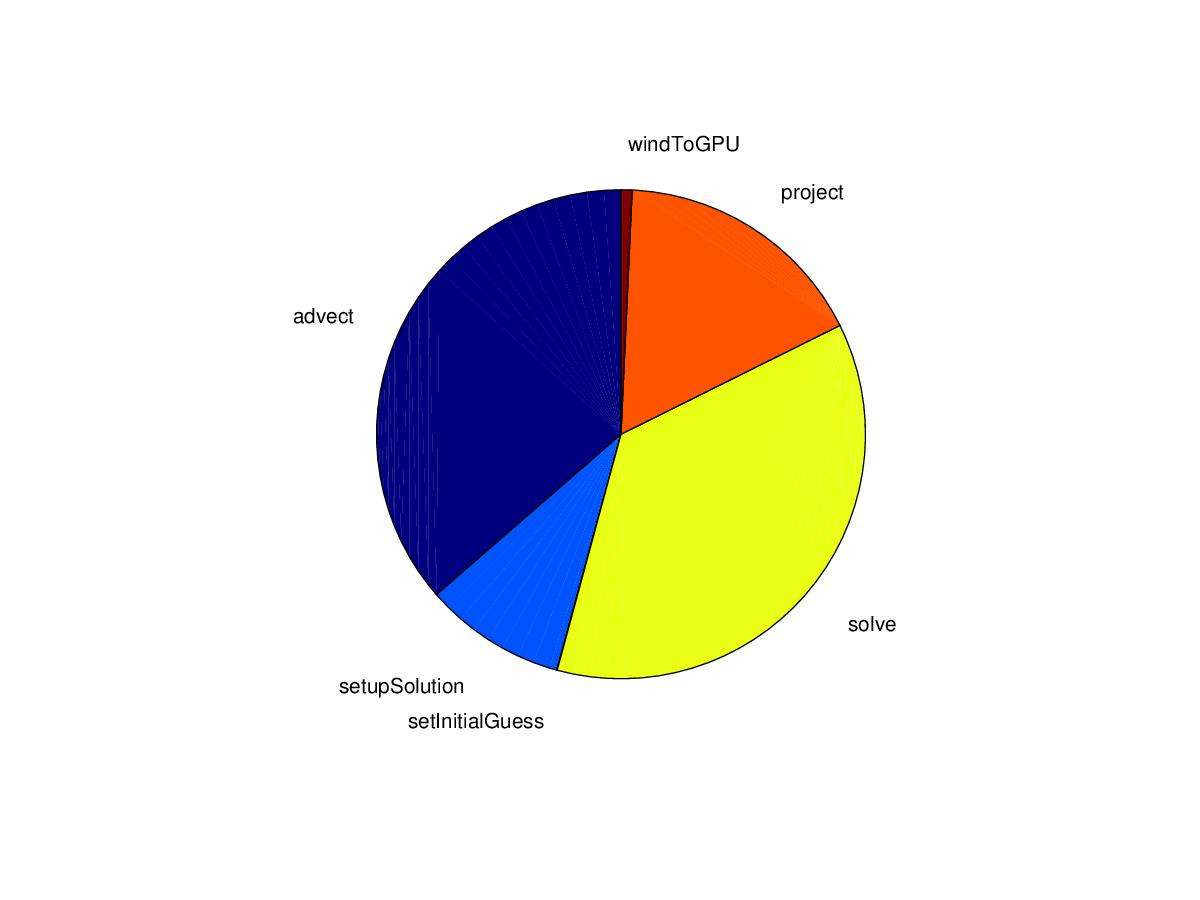
\includegraphics[width=1.0\textwidth]{results/data/td_conf1_petsc_cpu}
		\caption{PETSc on the CPU.}
		\label{fig:td_conf1_petsc_cpu}
	\end{subfigure}
	\caption{Time distribution of the execution time of the key functions
			with configuration 1}
	\label{fig:td_conf1}
	
\end{figure}

\begin{figure}[ht]
	\center
	
	\begin{subfigure}{0.45\textwidth}
		\center
		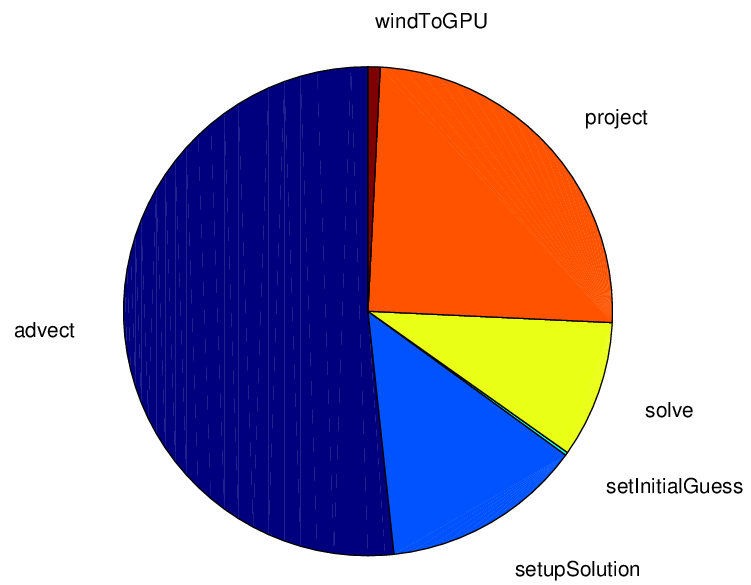
\includegraphics[width=1.0\textwidth]{results/data/td_conf2_petsc_gpu}
		\caption{PETSc on the GPU with OpenCL.}
		\label{fig:td_conf2_petsc_gpu}
	\end{subfigure}
	\begin{subfigure}{0.45\textwidth}
		\center
		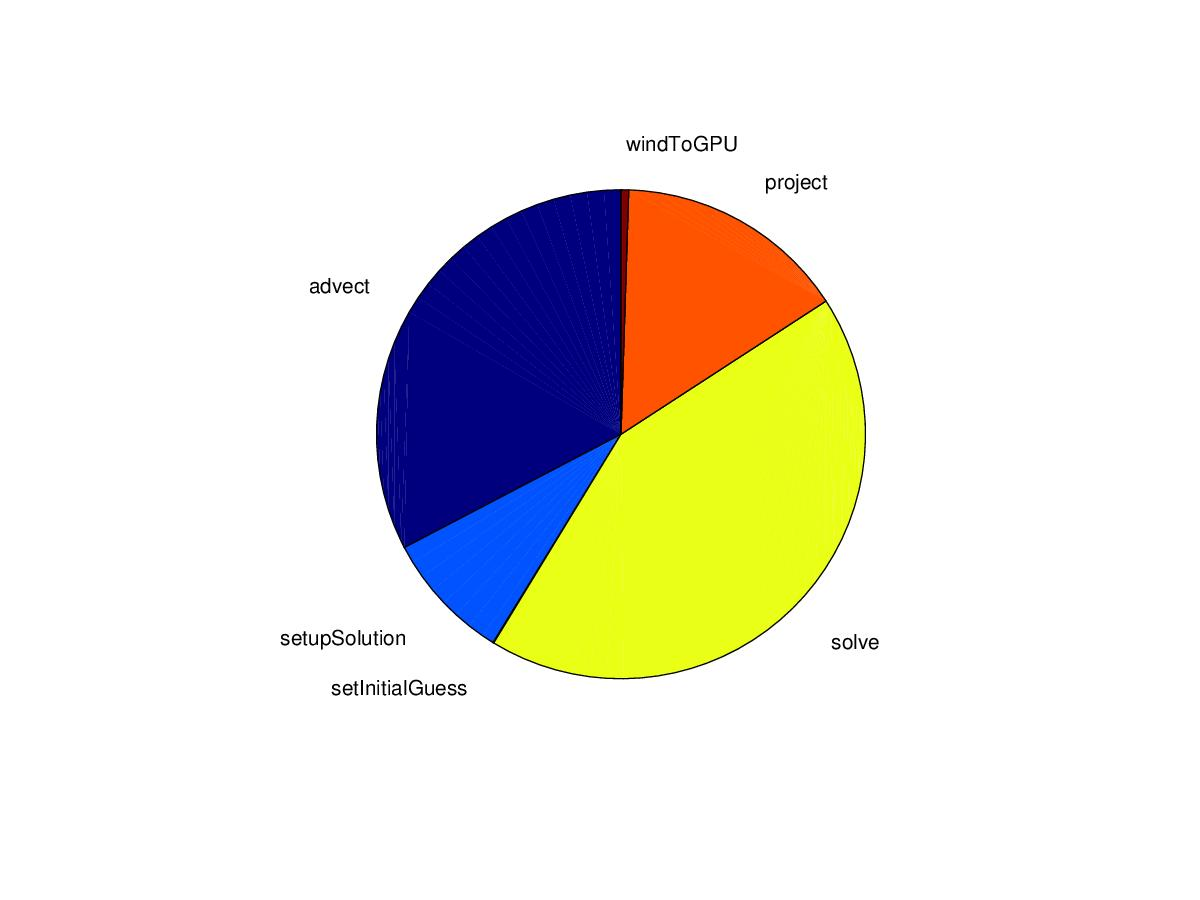
\includegraphics[width=1.0\textwidth]{results/data/td_conf2_petsc_cpu}
		\caption{PETSc on the CPU.}
		\label{fig:td_conf2_petsc_cpu}
	\end{subfigure}
	\caption{Time distribution of the execution time of the key functions
			with configuration 2}
	\label{fig:td_conf2}
	
\end{figure}

\begin{figure}[ht]
	\center
	
	\begin{subfigure}{0.45\textwidth}
		\center
		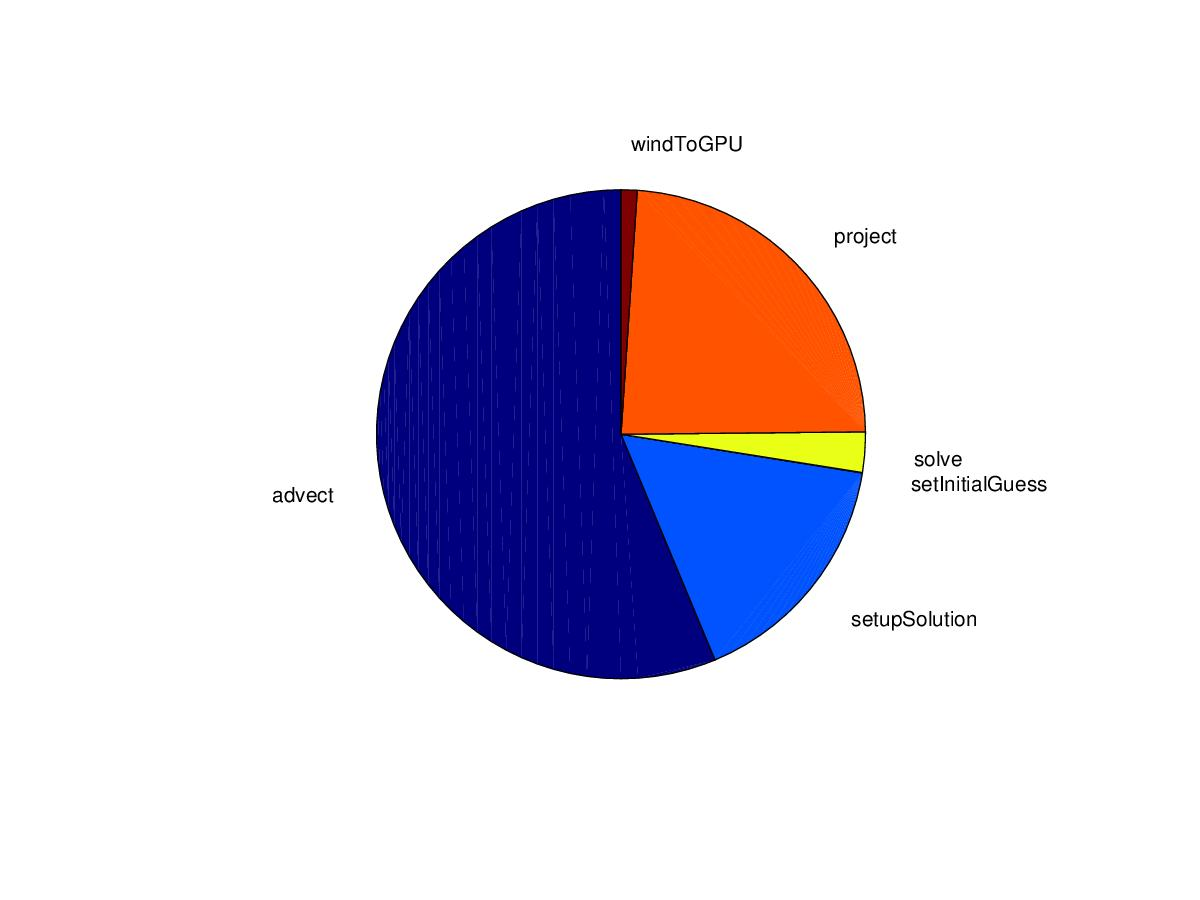
\includegraphics[width=1.0\textwidth]{results/data/td_conf3_petsc_gpu}
		\caption{PETSc on the GPU with OpenCL.}
		\label{fig:td_conf3_petsc_gpu}
	\end{subfigure}
	\begin{subfigure}{0.45\textwidth}
		\center
		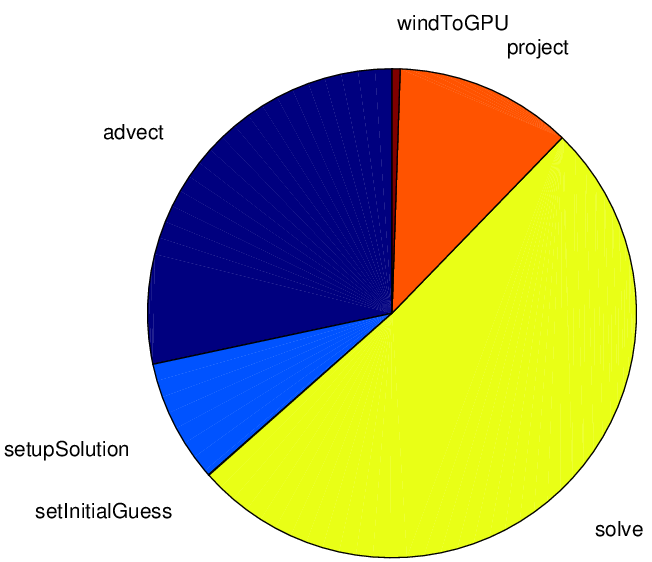
\includegraphics[width=1.0\textwidth]{results/data/td_conf3_petsc_cpu}
		\caption{PETSc on the CPU.}
		\label{fig:td_conf3_petsc_cpu}
	\end{subfigure}
	\caption{Time distribution of the execution time of the key functions
			with configuration 3}
	\label{fig:td_conf3}
	
\end{figure}

\begin{figure}[ht]
	\center
	
	\begin{subfigure}{0.45\textwidth}
		\center
		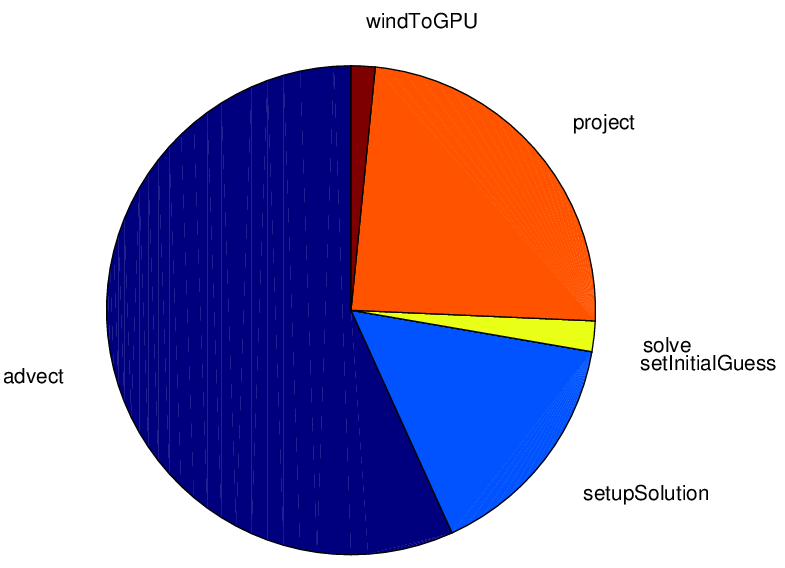
\includegraphics[width=1.0\textwidth]{results/data/td_conf4_petsc_gpu}
		\caption{PETSc on the GPU with OpenCL.}
		\label{fig:td_conf4_petsc_gpu}
	\end{subfigure}
	\begin{subfigure}{0.45\textwidth}
		\center
		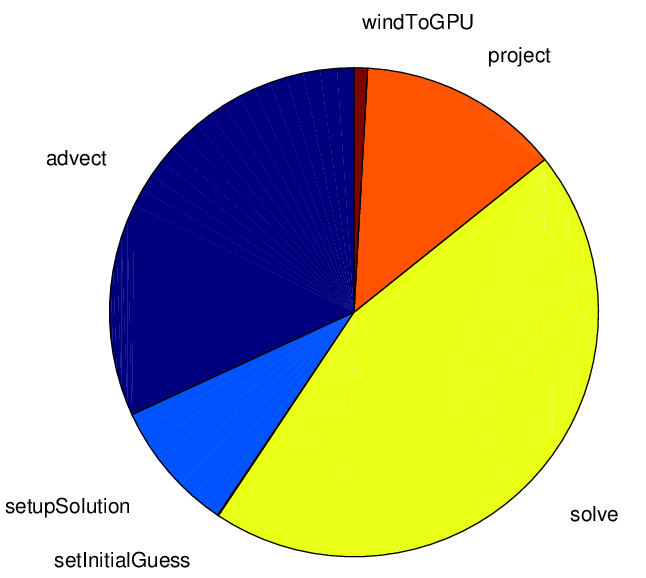
\includegraphics[width=1.0\textwidth]{results/data/td_conf4_petsc_cpu}
		\caption{PETSc on the CPU.}
		\label{fig:td_conf4_petsc_cpu}
	\end{subfigure}
	\caption{Time distribution of the execution time of the key functions
			with configuration 4}
	\label{fig:td_conf4}
	
\end{figure}

\subsection{Visual Results}

TODO: Show the windfield and pressure field and obstacle field (if I have time)
